\section{Corpus créé}%
\label{sec.results.corpus}

Après avoir construit le corpus parallèle en suivant la démarche décrite dans 
\Cref{sec.conception.archi,subsec.mt-corpus-creation},
il est nécessaire d'évaluer sa qualité.
Pour cela, nous avons choisi deux métriques : le score \gls{bleu} (voir Section~\ref{subsec.nmt.eval})
et la perplexité.

\subsection{Perplexité}%
\label{subsec.results.corpus.perplexity}

La perplexité est une mesure de la qualité d'un modèle de langue par rapport à un corpus.
Si la qualité du modèle est connue (et bonne), la perplexité est une mesure de la qualité du corpus.
La perplexité du corpus \(\mathcal{C}\) par rapport au modèle de langue \(\mathcal{M}\) est définie
comme la moyenne géométrique des probabilités des phrases du corpus (voir l'équation~\ref{eq.perplexity}).
\begin{equation}
  \label{eq.perplexity}
  \text{perplexité}(\mathcal{C}, \mathcal{M}) = 
  \prod_{s\in\mathcal{C}}\mathcal{M}(s)^{-\frac{1}{|\mathcal{C}|}}
\end{equation}

En prenant le logarithme de la perplexité, 
on retrouve l'entropie croisée de la loi de probabilité donnée par \(\mathcal{M}\) 
et celle induite par \(\mathcal{C}\)%
\footnote{À une constante multiplicative dépendante de la base du logarithme près}.
Elle mesure ainsi la dissimilarité entre ces deux lois (voir Section~\ref{subsec.nmt.eval}).
La perplexité des phrases générées (pour simuler l'aphasie de Broca) 
est une mesure de la dissimilarité entre ses phrases et le français courant.


\begin{figure}[hbt]
  \begin{center}
    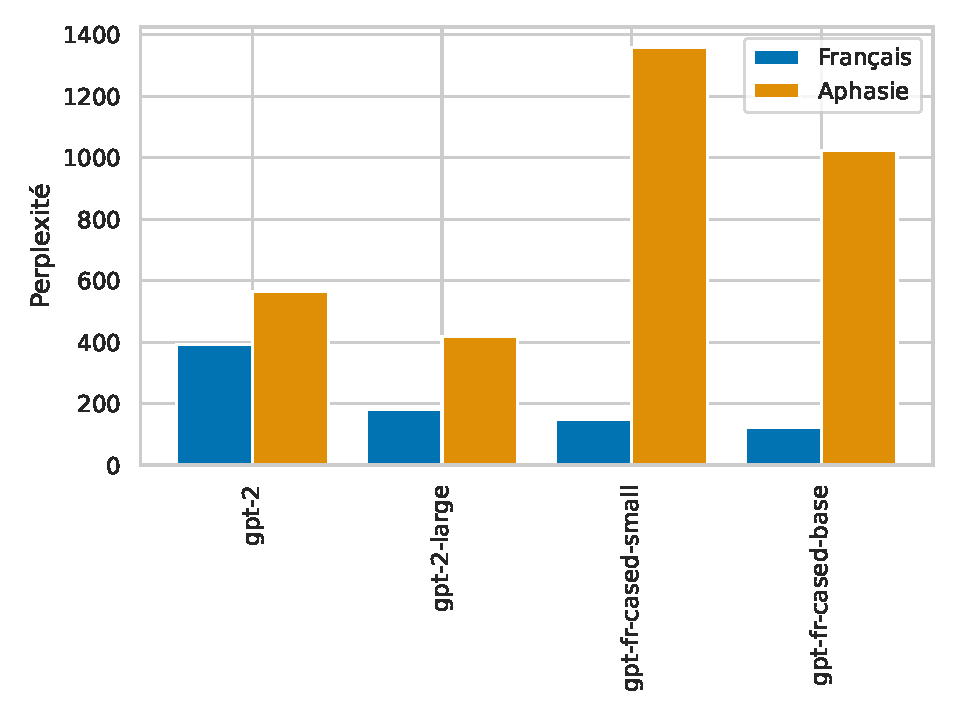
\includegraphics[width=.8\textwidth]{assets/python/perplexity.pdf}
  \end{center}
  \caption{Perplexité des phrases du corpus par rapport à différents modèles de langue.}
  \label{fig.perplexity}
\end{figure}
\begin{table}[hbt]
  \begin{center}
    \begin{tabular}{|l|c|c|}
      \cline{2-3}
      \multicolumn{1}{c|}{} &  french &  aphasia \\
      \hline
      \verb|gpt-2|              &  392.07 &   566.07 \\
      \hline
      \verb|gpt-2-large|        &  182.20 &   417.30 \\
      \hline
      \verb|gpt-fr-cased-small| &  147.84 &  1357.31 \\
      \hline
      \verb|gpt-fr-cased-base|  &  123.93 &  1023.12 \\
      \hline
      \end{tabular}
  \end{center}
  \caption{Perplexité des phrases du corpus par rapport à différents modèles de langue.}
  \label{tab.perplexity}
\end{table}


Pour calculer la perplexité, nous avons utilisé quatre modèles de langage basés sur \glsxtrshort{gpt}-2
et hébergés sur \foreignlanguage{english}{Hugging Face Hub} :
\begin{itemize}
  \item \cprotect{\href{https://huggingface.co/gpt2}}{\verb|gpt2|} : 
  ce modèle compte 124 M de paramètres et a été entraîné sur 40 Go de texte en plusieurs langues.
  \item \cprotect{\href{https://huggingface.co/gpt2-large}}{\verb|gpt2-large|} :
  ce modèle compte 774 M de paramètres et a été entraîné sur le même corpus que \verb|gpt2|.
  \item \cprotect{\href{https://huggingface.co/asi/gpt-fr-cased-small}}{\verb|gpt-fr-cased-small|} :
  ce modèle compte 124 M de paramètres et a été entraîné sur un corpus de textes en français d'une taille non précisée.
  \item \cprotect{\href{https://huggingface.co/asi/gpt-fr-cased-base}}{\verb|gpt-fr-cased-base|} :
  ce modèle compte 1.017 G de paramètres et a été entraîné sur le même corpus que \verb|gpt-fr-cased-small|.
\end{itemize}
Le code utilisé pour calculer la perplexité est donné par l'Extrait de code~\ref{code.perplexity}.
Ce code a été exécuté sur Google Colaboratory avec une instance GPU munie de 16 Go de mémoire vive.

Les résultats sont donnés par Figure~\ref{fig.perplexity} et Table~\ref{tab.perplexity}.
On y observe que tous les modèles attribuent une perplexité plus faible 
aux phrases en français qu'à celles qui simulent l'aphasie de Broca.
On note également que cette différence est plus prononcée pour les modèles entraînés sur des textes en français.

\begin{lstlisting}[
  language=Python,
  caption=Calcul de la perplexité avec le modèle \texttt{gpt-fr-cased-base}.,
  label={code.perplexity}
]
import pandas as pd
import evaluate

# Load perplexity metric
perplexity = evaluate.load("perplexity", module_type="measurement")

# Load data
df = pd.read_csv("val.csv")
fr = df.french.tolist()
aph = df.aphasia.tolist()

# Compute perplexities
fr = perplexity.compute(
  model_id='asi/gpt-fr-cased-base', 
  add_start_token=False, 
  data=fr
)
aph = perplexity.compute(
  model_id='asi/gpt-fr-cased-base', 
  add_start_token=False, 
  data=aph
)

print(f'{fr["mean_perplexity"]=:.2f}, {aph["mean_perplexity"]=:.2f}')
\end{lstlisting}

Les différences données par ces derniers sont compatibles avec les résultats obtenus 
par~\cite{ghumman2021training} avec des transcriptions de patients aphasiques et un groupe de contrôle.
Il est raisonnable d'en conclure que les phrases générées sont similaires 
à celles produites dans le cas d'une aphasie de Broca.

\subsection{Score \glsfmtshort{bleu}}%
\label{subsec.results.corpus.bleu}

Le problème avec l'utilisation de la perplexité pour mesurer 
la différence entre les phrases générées et le langage ordinaire,
est qu'elle ne prend pas en compte la relation entre une phrase aphasique et la phrase correcte qui lui correspond. 
Elle traite les deux corpus comme étant indépendants.
\gls{bleu} est une métrique qui prend en compte cette relation (voire Section~\ref{subsec.nmt.eval}).
En prenant la moyenne des scores \gls{bleu} de chaque couple de phrases dans le corpus parallèle,
nous obtenons un seul nombre qui mesure la similarité entre les deux parties du corpus.

L'Extrait de code~\ref{code.bleu} donne le code utilisé pour calculer le score \gls{bleu}.
La fonction \verb|bleu_score| de \verb|torchmetrics| prend en entrée 
une liste de phrases qui représentent les traductions candidates (dans notre cas, les phrases aphasiques)
et une liste de listes de phrases qui représentent les traductions de référence (dans notre cas, les phrases en français).
L'exécution de ce code donne un score \gls{bleu} de \(62.72\%\) sur le corpus de validation.
\begin{lstlisting}[
  language=Python,
  caption=Calcul du score \texttt{BLEU} sur le corpus de validation.,
  label={code.bleu}
]
import pandas as pd
from torchmetrics.functional import bleu_score

df = pd.read_csv("val.csv")

aphasia = df.aphasia.to_list()
french = df.french.tolist()

french = [[s] for s in french]
score = bleu_score(aphasia, french) * 100
print(f"{score=:.2f}%")
\end{lstlisting}
